\begin{figure}[ht]
	\begin{subfigure}[b]{0.32\linewidth}
		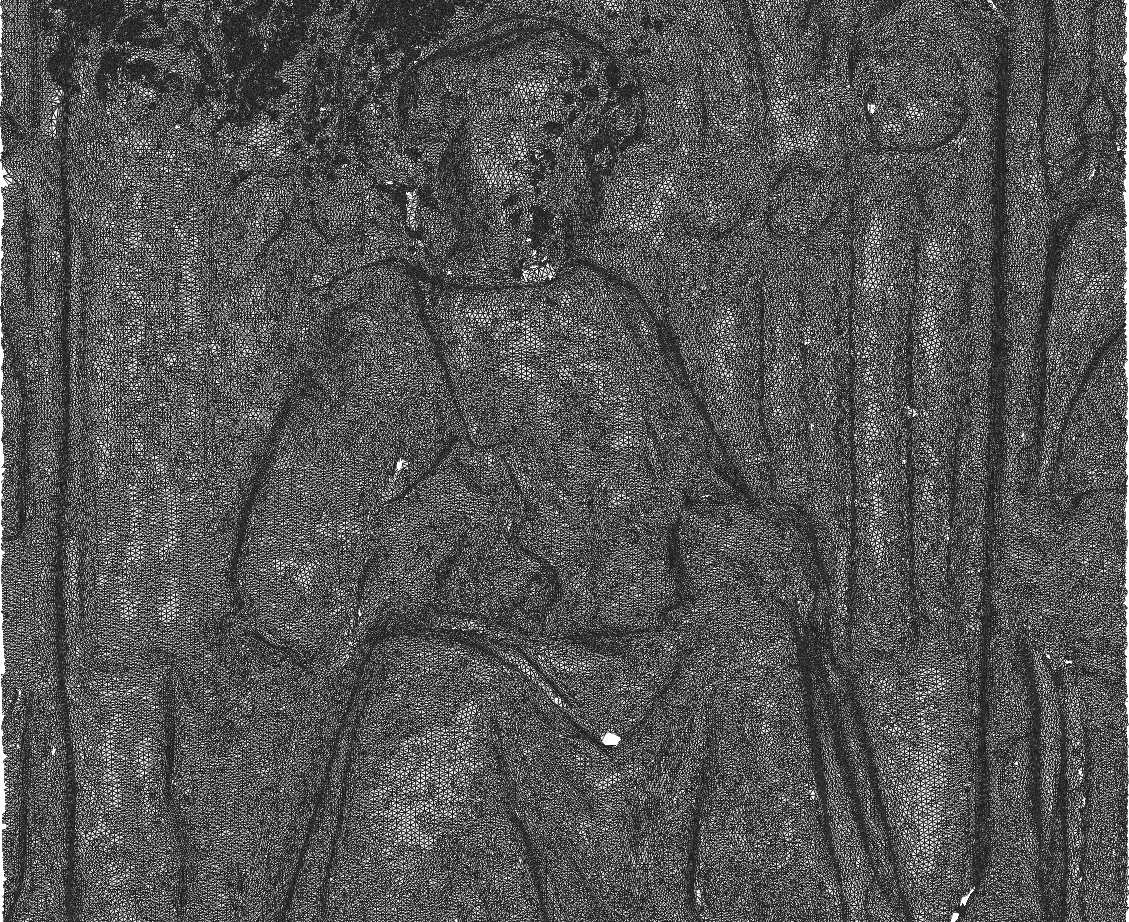
\includegraphics[width=\linewidth]
		{data/acquired_meshes/unisiegel_wireframe.png}
		\caption{wireframe}\label{fig:bun.a}
	\end{subfigure}
	\begin{subfigure}[b]{0.32\linewidth}
		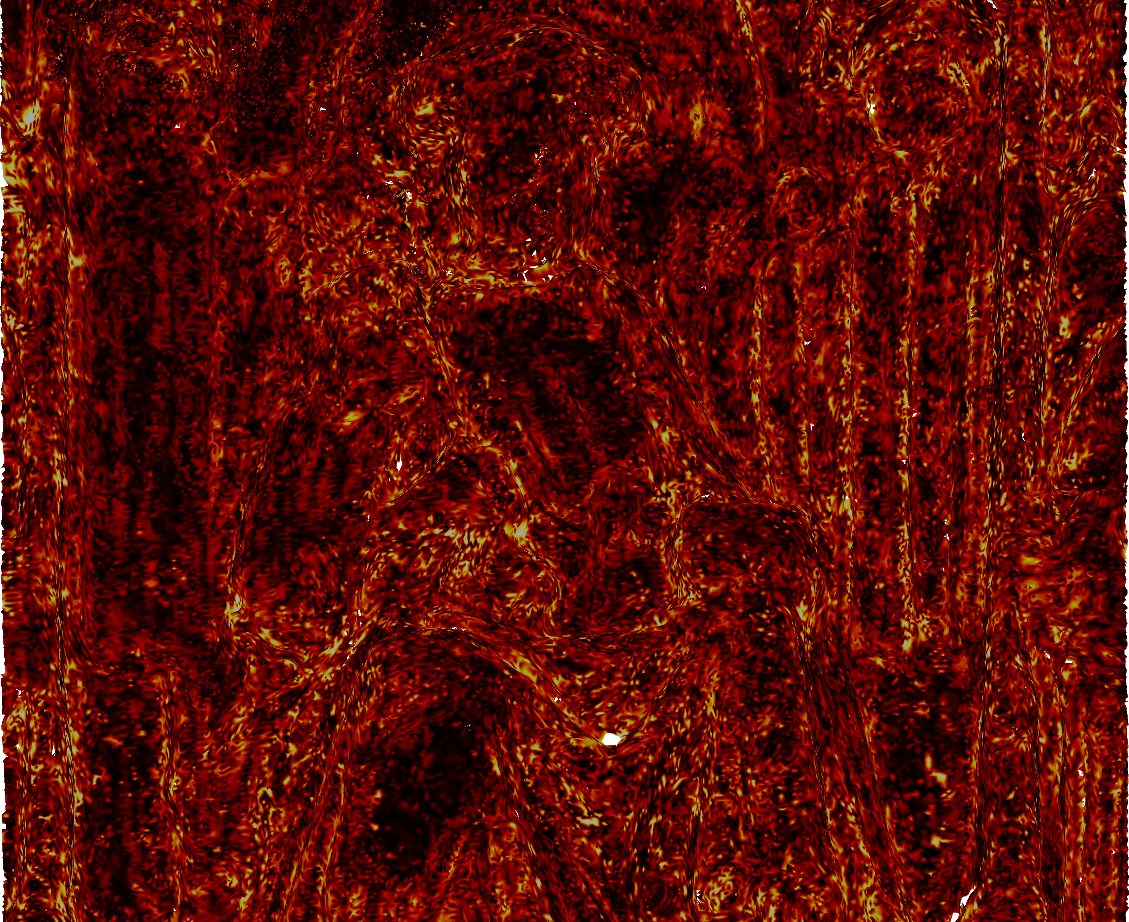
\includegraphics[width=\linewidth]
		{data/acquired_meshes/unisiegel_0iter.png}
		\caption{$c=0$}\label{fig:bun.b}
	\end{subfigure}
	\begin{subfigure}[b]{0.32\linewidth}
		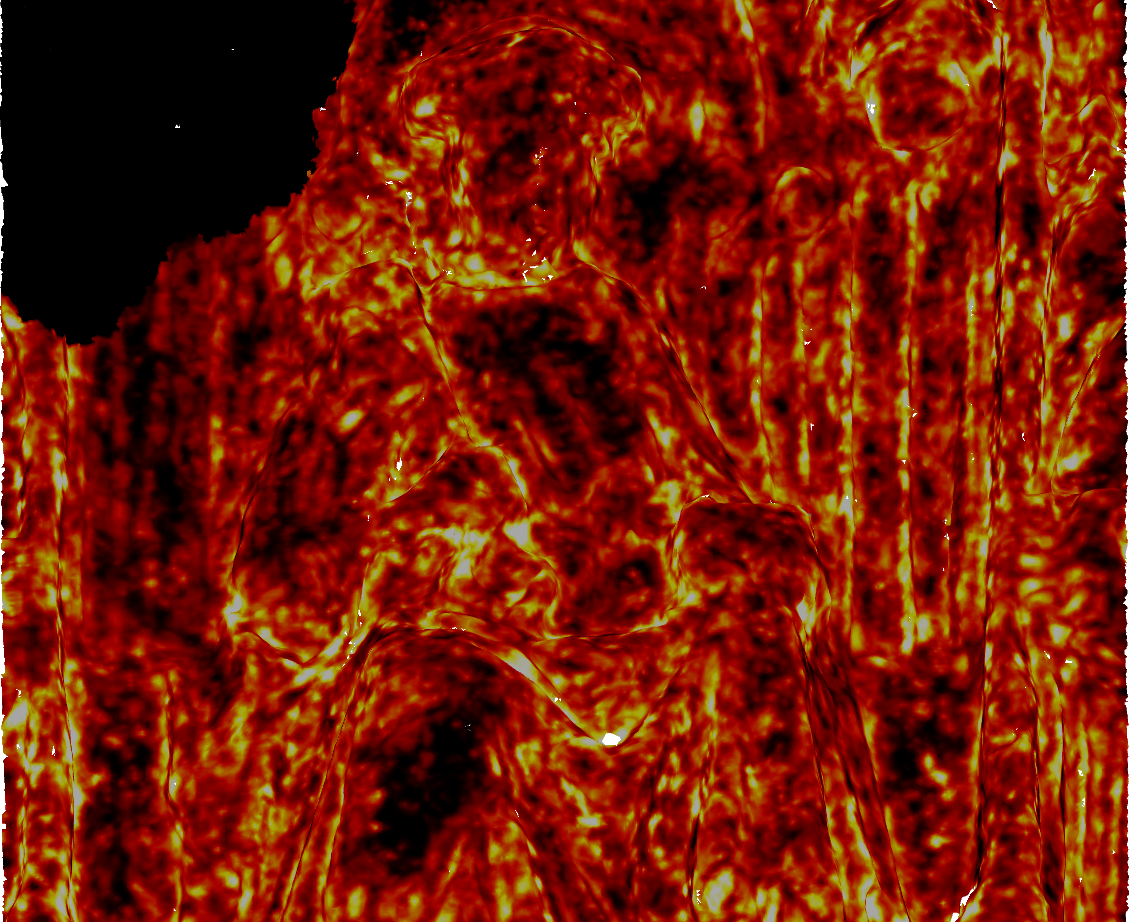
\includegraphics[width=\linewidth]
		{data/acquired_meshes/unisiegel_100iter.png}
		\caption{$c=100$}\label{fig:bun.c}
	\end{subfigure}
	\caption[Three views of the Stanford Bunny]{Three views of the Stanford Bunny (a) in wireframe (b) colored by MSII function value before convolving the filter (c) colored by function value after convolving the filter 100 times.}
	\label{fig:bun}
\end{figure}
\todoCitation{}
